\documentclass{article}
\usepackage[T1]{fontenc}
\usepackage{template/spconf,amsmath,graphicx,booktabs,url}
\setlength{\emergencystretch}{2em}
\title{Auditing and Extending Edge-Enhanced Nucleus Segmentation:\\Matched-Budget Learning and Breast Histology Transfer}
\name{Varun Kumar Dasoju$^{1}$, Qingsu Cheng$^{2}$, and Zeyun Yu$^{1}$}
\address{University of Wisconsin--Milwaukee, Milwaukee, WI, USA\\
$^{1}$Department of Computer Science; $^{2}$Department of Biomedical Engineering\\
\textit{Discussion draft, 29 September 2026 --- author approval and metadata pending}}
\begin{document}
\maketitle
\begin{abstract}
Edge-enhanced nuclear segmentation promises annotation-efficient microscopy analysis, but improvements require fair controls and cross-domain evaluation. We revisit a mammary epithelial nucleus pipeline using Gabor features, an EfficientNet-B7 encoder, UNet++, attention and a learned input projection. An implementation audit motivates stable preprocessing, complete validation and explicit boundary evaluation. Seven configurations are compared across three seeds on the official BBBC039 split and transferred to breast histology. Vanilla B7 and the Gabor bundle achieve 96.60\% and 96.85\% mean test Dice. An identity-preserving residual alternative reaches 96.57\%, without improving the Gabor bundle. That bundle achieves only 2.94\% patient-macro Dice on TNBC without histology training. Earlier private and volumetric results remain provenance-limited context. These findings support a small within-domain gain but not broad generalization, instance-separation superiority or clinical cancer detection. Independent confirmation remains necessary.
\end{abstract}
\begin{keywords}
Nucleus segmentation, Gabor features, reproducibility, boundary evaluation, domain shift
\end{keywords}

\section{Introduction}
\label{sec:intro}
This work continues a project on annotation-limited mammary epithelial nuclear segmentation. Its original design combines oriented Gabor features with a pretrained EfficientNet-B7 encoder, a nested UNet++ decoder, and spatial/channel squeeze-and-excitation (SCSE). The relevant question is whether these additions improve a well-trained control and transfer to independently sourced images, rather than whether a complex pipeline exceeds weak historical baselines.

U-Net introduced an effective encoder--decoder with skip connections~\cite{unet}, UNet++ developed nested decoding~\cite{unetpp}, and EfficientNet provides compound-scaled pretrained encoders~\cite{effnet}. Cross-experiment nucleus benchmarks emphasize imaging diversity~\cite{dsb}. Cellpose-SAM is an off-the-shelf reference~\cite{cpsam}; recent microscopy foundation models also include $\mu$SAM~\cite{microsam} and CellSAM~\cite{cellsam}, which are not newly evaluated here. Their pretraining and task-specific adaptation must be distinguished from matched-data learning. Breast histology introduces stain and tissue-context shifts~\cite{naylor}. High overlap on private slices therefore does not establish cancer-detection performance.

We retain the original method and its 2D-to-3D progression while auditing its evidence. Our contributions are an auditable implementation, matched-budget controls separating projection, attention, edge choice and boundary loss, and complete public-data transfer evaluation including failures. Zero-initialized residual edge fusion is tested as an engineering hypothesis, not asserted as a uniquely novel architecture. The experiments are exploratory because prior public test results informed development; checkpoints within each run are selected only on validation data.

\section{Original pipeline and corrected method}
\subsection{Retaining the original method}
The original fourth channel is the maximum absolute response from 24 Gabor kernels: eight orientations $\theta\in[0,\pi)$ and three frequencies $f\in\{0.05,0.15,0.25\}$ cycles per native pixel. Kernels have size 31, $\sigma=5$, aspect ratio $\gamma=0.5$ and zero phase. A convolutional $4\!\to\!16\!\to\!8\!\to\!3$ projection feeds EfficientNet-B7/UNet++/SCSE. Adaptive loss and complexity-based sampling motivated the original training recipe; their earlier private-data ablations are retained in the accompanying research package.

The two supplied code exports differ: the newer nested export fixes the older ignored sampling flag. Both retain validation filtering and logits/probability range guessing. Stored proposed-model Dice and IoU means exceed the means of their saved per-image values by exactly 0.01. Those aggregates are not adopted as validated results. The intervening corrected private-data study, including 34 architecture, edge, encoder, loss and sampling conditions, is preserved separately from the new public experiments.

\subsection{Preprocessing and identity-preserving fusion}
Images retain native intensity precision until grayscale conversion and rescaling between their first and 99.5th percentiles. Grayscale is replicated into three image channels. Gabor kernels are normalized by their L1 norm, replacing unstable signed-sum normalization:
\begin{equation}
 e(x)=\mathcal N\!\left(\max_{\theta,f}\left|x*\frac{k_{\theta,f}}{\|k_{\theta,f}\|_1+\epsilon}\right|\right),
\end{equation}
where $\mathcal N$ maps the response to $[0,1]$. Image and edge channels are resized to $512\times512$ and standardized; image channels use ImageNet means/standard deviations and the edge uses 0.5/0.25. Sobel magnitude is an alternative edge input under the same normalization. Preprocessing is identical at training and inference.

Vanilla B7 has neither SCSE nor the edge projection. The Gabor bundle adds both; this is not an isolated Gabor comparison. SCSE-only supplies an attention control. Residual fusion instead uses
\begin{equation}
 x_{\mathrm{out}}=x_{\mathrm{RGB}}+\tanh(a)P([x_{\mathrm{RGB}},e]),\quad a_0=0.
\end{equation}
The pretrained encoder therefore initially receives the unchanged standardized image. Residual Gabor/Sobel variants have identical initial weights within each seed. A small learned scalar alone is not proof that the branch is unnecessary or causal.

\subsection{Explicit boundary objective}
All public models use
\begin{equation}
 \mathcal L=0.5\mathcal L_D(p,y)+0.5\mathcal L_{\mathrm{BCE}}(z,y)
 +\lambda\mathcal L_D(B(p),B(y)),
\end{equation}
where $p=\operatorname{sigmoid}(z)$, $\mathcal L_D$ is samplewise soft Dice loss with numerator/denominator smoothing 1, and $B(u)=\operatorname{maxpool}_3(u)-\operatorname{minpool}_3(u)$. Boundary variants use $\lambda=0.1$; others use zero. Unlike overlap-only Tversky, this explicitly involves boundaries. No recall-bias claim is made. Uniform sampling and this common objective are disclosed protocol changes, not an exact retraining of the submitted recipe.

\section{Experimental design}
\subsection{Public datasets and original breast-cell context}
BBBC039v1 has 200 native $520\times696$, 16-bit U2OS fluorescence fields, one per compound from one chemical screen~\cite{bbbc}. We use its official 100/50/50 training/validation/test partition and the provider's red-channel foreground decoding. Identifiers, field groups and decoded-image hashes are checked for cross-partition overlap. These are not breast cells or independent clinical patients. No ROI extraction or crop generation is used.

All new models transfer without tuning to all 50 TNBC breast-histology images from 11 patient groups~\cite{naylor}. The released binary masks support semantic foreground, not touching-instance counts. Earlier frozen-model evaluations on BBBC038 (65 images), BBBC039 (50) and TNBC (50) are retained. BBBC039 partly overlaps BBBC038, so newly BBBC039-trained models are not claimed to have independent BBBC038 validation. Foundation-model pretraining overlap is unresolved.

The earlier corrected private study has 855 valid foreground-containing images; 334 are traceable to eight stacks and 521 lack exact source matching. Its conservative shape-group split has 516/133/206 images. Shape groups are not verified independent biological volumes. Acquisition, annotation agreement, physical calibration and release metadata remain author-completion items. Its results provide exploratory lineage rather than the main confirmatory evidence.

\subsection{Matched training and evaluation}
Each configuration uses seeds 0/1/2, ImageNet encoder initialization, a random decoder, AdamW (learning rate $3\cdot10^{-4}$, weight decay $10^{-4}$), batch size 8, gradient clipping at 1, and 20 epochs with cosine decay to 1\% of the initial learning rate. Augmentations are rotations by multiples of $90^\circ$ and horizontal flips with probability 0.5. Bfloat16 autocast uses float32 loss. The final short batch is retained; nonfinite loss/gradients stop training. The highest complete native-grid validation mean Dice selects the checkpoint. There is no metric smoothing, outlier exclusion, TTA, or test-based threshold selection.

Probabilities are bilinearly restored to native grids and thresholded at 0.5. Endpoints are Dice, IoU, boundary F1 (BF1) and surface Dice within two native pixels, and pooled bidirectional HD95. Both-empty pairs score overlap/boundary 1 and HD95 0; one-empty pairs score overlap/boundary 0 with image-diagonal HD95. Empty flags are retained. All evaluated public references contain foreground, so true-empty specificity remains untested. Distances are pixels, not micrometres.

Seed SD describes run variation. For paired inference, seed scores are averaged within each field before 10,000 bootstrap resamples and two-sided Wilcoxon tests. Ten contrasts by two endpoints form one Holm-corrected family per dataset. TNBC first averages images within each patient. Seeds are not independent patients, and seed-score averaging is not prediction ensembling. BBBC039 field-level inference is descriptive within one acquisition study. Initial conditions were planned together; four follow-up conditions were designed after initial seed-0 results, not as independent confirmation.

\section{Results}
\begin{table}[t]
\centering\small
\caption{New public training: three-seed means. Dice shows seed SD. BF1 uses two native pixels. TNBC is patient-macro transfer, not histology-trained performance.}
\label{tab:main}
\resizebox{\columnwidth}{!}{\begin{tabular}{@{}lrrr@{}}\toprule
Model & Dice (\%) & BF1 (\%) & TNBC (\%)\\\midrule
Vanilla B7 & 96.60 $\pm$ 0.07 & 98.53 & 8.07 \\
Gabor bundle & 96.85 $\pm$ 0.13 & 98.63 & 2.94 \\
Gabor + boundary & 96.84 $\pm$ 0.05 & 98.68 & 3.86 \\
SCSE-only B7 & 96.38 $\pm$ 0.53 & 98.48 & 4.36 \\
Residual Gabor & 96.57 $\pm$ 0.27 & 98.52 & 4.04 \\
Residual Sobel & 96.44 $\pm$ 0.48 & 98.47 & 4.43 \\
Residual Gabor + boundary & 96.61 $\pm$ 0.31 & 98.58 & 4.49 \\
\bottomrule\end{tabular}}
\end{table}

\subsection{Matched public training and transfer}
Table~\ref{tab:main} reports all seven configurations (21 runs, 420 epochs). Residual Gabor changes Dice by -0.28 percentage points relative to the original random-projection Gabor bundle and -0.03 points relative to vanilla B7. The configuration with the highest mean selected-validation score is Gabor + boundary, yielding 96.84\% test Dice; this is not selection of the highest test score. Full per-image metrics, learning curves and adjusted comparisons accompany the research package.

Gabor versus vanilla gives a 0.250-percentage-point Dice difference (descriptive paired-field bootstrap 95\% interval [0.197, 0.299]; $p_{\mathrm{Holm}}=7.34\times10^{-9}$). This small within-screen effect is not an acquisition-level confidence statement or proof of clinical value; paired field inference averages seeds and does not capture a large population of training runs.

\begin{figure}[t]
\centering
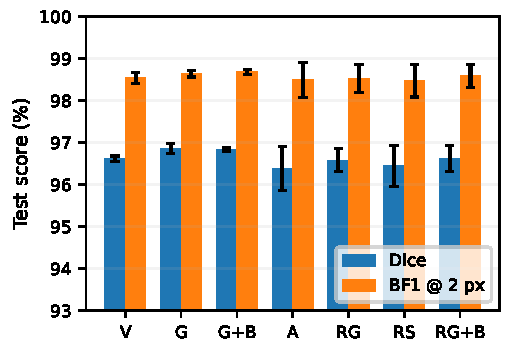
\includegraphics[width=\columnwidth]{../reports/figures/paper_results.pdf}
\caption{Native-grid BBBC039 test scores. V: vanilla; G: Gabor; B: boundary loss; A: SCSE-only; RG/RS: residual Gabor/Sobel. Error bars are seed SD; truncated vertical scale shows small differences. Complete learning curves are retained in the research package.}
\label{fig:curves}
\end{figure}

All new checkpoints are also evaluated on the complete TNBC set without adaptation. Residual Gabor reaches 4.04\% patient-macro Dice. Grayscale fluorescence training and H\&E breast histology differ substantially; this is a domain-transfer stress test, not a matched histology-training leaderboard. The data do not establish cancer diagnosis or pathologist-validated morphometry.

The earlier released and revised checkpoints score 32.66 and 71.67\% Dice on BBBC038, 92.04 and 91.58\% on BBBC039, and 21.08 and 17.55\% on TNBC (image-macro). Cellpose-SAM scores 87.02, 96.95 and 82.13\%, respectively, as an off-the-shelf reference with unresolved pretraining overlap. Otsu scores 75.45, 94.79 and 42.75\%. These frozen-model results are not merged with new training or patient-macro aggregation. An additional audit evaluates all 24 supplied historical checkpoints on all three complete partitions; failures and weak outcomes are retained rather than omitted. Historical unequal training cannot establish method superiority.

\subsection{Original private and exploratory 3D results}
The previous corrected private study reports group-macro Dice 0.9312 for the full model, 0.9349 for vanilla B7, 0.9320 for U-Net ResNet-50 and 0.9366 for a plain Dice+BCE ablation, without a significant full-model advantage after multiplicity correction. Its Gabor sensitivity and smaller-encoder controls remain in the extended package, subject to unresolved biological source groups.

Existing volumetric work evaluates 334 annotated planes from eight traceable stacks. Stack-macro Dice is 0.9181 for fixed Cellpose-SAM, 0.8580 for fixed-threshold distilled 3D U-Net, 0.9137 for nested-selected U-Net/fusion and 0.9177 for nested Cellpose-plus. These selected-plane semantic scores do not establish dense 3D instance accuracy or improvement over Cellpose. QC-student pseudo-label validation is not human-reference evidence.

\section{Discussion and conclusion}
The original edge-enhanced method is preserved while its evidence is made more auditable. Architectural controls, complete validation and explicit boundary metrics distinguish possible improvements from evaluation artifacts. A residual input path addresses the concern that random projection changes the input distribution of a pretrained encoder; its value must still be judged against attention-only and alternative-edge controls. The boundary term likewise requires measured benefit, not a claim inferred from its name.

The Gabor bundle modestly exceeds vanilla under matched training, but residual fusion does not improve that bundle and the added boundary term does not establish a Dice gain over it. Cellpose-SAM's 96.95\% BBBC039 Dice remains above the Gabor mean, with unequal pretraining. The new architecture therefore should not replace the original on the assumption that added complexity is beneficial.

Limitations include a single chemical-screen acquisition, three seeds, a short fixed training budget, prior test exposure, no full public data-efficiency curve, and unresolved private annotation/source metadata. Existing private Gabor/encoder sweeps require public-protocol replication. Binary foreground masks do not support instance-AP or split/merge conclusions. Neither within-screen significance nor a zero-initialized residual design establishes unique algorithmic novelty or clinical utility.

The next decisive experiment is patient-separated histology adaptation followed by a genuinely unexamined breast cohort, with a prespecified endpoint and matched modern baselines. Public code, permissible weights and source manifests are necessary for independent reproduction. The present result is a controlled continuation of the original 2D project with a bounded 3D extension, not a guaranteed state-of-the-art or clinical claim.

\section{Compliance with ethical standards}
\textbf{Author completion required.} BBBC038/039 are CC0 and TNBC is CC BY 4.0. Public licensing does not determine institutional ethics requirements. Authors must confirm public-reuse and original cell-line ethics or exemption wording, annotation provenance, private-data permissions and any applicable approval identifiers. This draft is not ready for submission until those statements are completed.

\section{Acknowledgments and availability}
\textbf{Author completion required:} authorship approval, funding and competing interests. Working code and result tables: \url{https://github.com/vkd14/breast-seg-isbi2027} (initially private; unrestricted release and weight archiving pending). Draft disclosure: OpenAI Codex assisted with code auditing, experimental scripting, analysis and methods/results/discussion drafting. Authors must independently validate all content. Figures use actual data and predictions, not generated microscopy imagery.

\begin{thebibliography}{9}
\bibitem{unet} O. Ronneberger, P. Fischer, and T. Brox, ``U-Net: Convolutional networks for biomedical image segmentation,'' in \emph{MICCAI}, 2015.
\bibitem{unetpp} Z. Zhou et al., ``UNet++: A nested U-Net architecture for medical image segmentation,'' in \emph{DLMIA}, 2018.
\bibitem{effnet} M. Tan and Q. Le, ``EfficientNet: Rethinking model scaling for convolutional neural networks,'' in \emph{ICML}, 2019.
\bibitem{dsb} J. C. Caicedo et al., ``Nucleus segmentation across imaging experiments: the 2018 Data Science Bowl,'' \emph{Nature Methods}, 2019, doi:10.1038/s41592-019-0612-7.
\bibitem{cpsam} M. Pachitariu, M. Rariden, and C. Stringer, ``Cellpose-SAM: superhuman generalization for cellular segmentation,'' \emph{bioRxiv}, 2025, doi:10.1101/2025.04.28.651001. Evaluated checkpoint: cpsam\_v2.
\bibitem{naylor} P. Naylor et al., ``Segmentation of nuclei in histopathology images by deep regression of the distance map,'' \emph{IEEE TMI}, 2019, doi:10.1109/TMI.2018.2865709. Data: doi:10.5281/zenodo.2579118.
\bibitem{bbbc} Broad Bioimage Benchmark Collection, ``BBBC039v1: Nuclei of U2OS cells in a chemical screen,'' \url{https://bbbc.broadinstitute.org/BBBC039}.
\bibitem{microsam} A. Archit et al., ``Segment Anything for Microscopy,'' \emph{Nature Methods}, vol. 22, pp. 579--591, 2025, doi:10.1038/s41592-024-02580-4.
\bibitem{cellsam} M. Marks et al., ``CellSAM: a foundation model for cell segmentation,'' \emph{Nature Methods}, vol. 22, pp. 2585--2593, 2025, doi:10.1038/s41592-025-02879-w.
\end{thebibliography}
\end{document}
